%%{ DOC HEAD

\pdfoutput=1
\documentclass[a4paper,12pt,titlepage, twoside]{article}
\usepackage[english]{babel}
\usepackage[utf8]{inputenc}
\usepackage{amssymb,amsmath}
\usepackage{algorithm,algpseudocode}
\usepackage[title,titletoc]{appendix}
\usepackage{latexsym}
\usepackage{a4wide}
\usepackage{color}
\usepackage{indentfirst}
\usepackage{graphicx}       %%% graphics for dvips
\usepackage{fancyhdr}
\usepackage{longtable}
\usepackage{pifont}
\usepackage{makeidx}
\usepackage{lastpage}
\usepackage{multirow}
\usepackage{dcolumn}
\usepackage{epstopdf}
\usepackage{url}
\usepackage{listings}
\usepackage{caption}
\usepackage{subcaption}
\usepackage{relsize}
\usepackage{pdfpages}
\usepackage{url}

%%{ custom macros

\newcommand{\unit}[2]{$#1~\ensuremath{\mathrm{#2}}$}
\newcommand{\strong}[1]{\textbf{#1}}
\newcommand{\coord}[1]{\textbf{#1}}
\newcommand{\norm}[1]{\left\lvert#1\right\rvert}
\newcommand{\m}[1]{\ensuremath{\mathbf{#1}}}
\newcommand\numberthis{\addtocounter{equation}{1}\tag{\theequation}}
\newcommand{\corrected}[1]{{\color{black} {#1}}}
\newcommand{\updated}[1]{{\color{black} {#1}}}

%%}

\newcommand{\Author}{Ing. Tomáš Báča}
\newcommand{\Supervisor}{Ing. Martin Saska, Dr. rer. nat.}
\newcommand{\Title}{Distributed Sensing with Group of Unmanned Aerial Vehicles}
\newcommand{\DocName}{Thesis}
\newcommand{\Keywords}{mobile robotics}
\newcommand{\Date}{1/1/2019}
\newcommand{\DOCVersion}{0.1}

\def\clinks{false}

\lstset{breaklines=true,captionpos=b,frame=single,language=sh,float=h}
\lstloadlanguages{sh,c}
\def\lstlistingname{Listing}%{Výpis}
\def\lstlistlistingname{Listings}%{Seznam výpisů}

% European layout (no extra space after `.')
\frenchspacing

% no indent, free space between paragraphs
\setlength{\parindent}{1cm}
\setlength{\parskip}{1ex plus 0.5ex minus 0.2ex}

\pagestyle{fancy}
\setlength{\headheight}{18pt}
\renewcommand{\footrulewidth}{0.4pt}

%\lfoot{ČVUT FEL, Katedra Kybernetiky, Gerstner Laboratory}
\cfoot{}
%\rfoot{\thepage$/$\pageref{LastPage}}

\fancypagestyle{plain}

\fancyhead[R]{}

\begin{document}

\pagestyle{fancy}
\pagenumbering{roman}
\cfoot{\thepage}
\tableofcontents
\pagenumbering{arabic}
\cleardoublepage

%%}

%%{ INTRODUCTION

\section{Introduction}

%%}

%%{ IONIZING RADIATION IMAGING

\section{Radiation imaging and dosimetry}

%%{ RADIATION DETECTORS

\subsection{Radiation detectors}

%%{ SCINTILLATING DOSIMETERS

\subsubsection{Scintillating dosimeters}

%%}

%%{ CCD DETECTORS

\subsubsection{CCD detectors}

%%}

%%{ TIMEPIX DETECTOR

\subsubsection{Timepix detector}

%%}

%%}

%%{ RADIATION IMAGING TECHNIQUES

\subsection{Radiation imaging techniques}

%%{ CODED APERTURES

\subsubsection{Coded apertures}

%%}

%%{ PINHOLE CAMERAS

\subsubsection{Pinhole cameras}

%%}

%%{ PINHOLE CAMERAS

\subsubsection{X-Ray Optics}

%%}

%%{ COMPTON CAMERAS

\subsubsection{Compton cameras}

%%}

%%}

%%}

\clearpage

%%{ GAMMA-RAY CAMERA

\section{Compton $\gamma$-ray camera}

%%{ INTERACTION OF IONIZING RADIATION WITH MATTER

\subsection{Interaction of ionizing radiation with matter}

%%{ DIFFERENTIAL CROSS SECTION

\subsubsection{Differential cross section}

In a classical mechanics, the properties of non-elastic scattering of a particle from an object (scattering center) are described by a differential cross section.
A total cross section characterizes an effective area of an event (collision, scattering).
For simulating the interaction of X-Ray and $\gamma$-Ray photons with matter, differential and total cross sections of the interaction need to be derived.

I am considering a single particle on an incident trajectory with the scattering object.
The displacement $b$ of the particle from the path to the scattering center is called the impact parameter, the radial angle of scattering is denoted as $\theta$.
Various types of reactions have a distinct relation between $b$ and $\theta$.
The total area of the impact parameter is the impact cross section $\sigma$, which can be obtained by integrating the impact parameter $b$ over all possible azimuthal angles $\phi$:
\begin{equation}
  \sigma\left(b\right) = \int_\Phi b\left(\phi\right)\,d\phi.
\end{equation}
In a case where the scattering does not influence $\phi$ (axially symmetrical case), the impact cross section takes following form
\begin{equation}
  \sigma\left(b\right) = \int_\Phi b\,d\phi = \frac{b^{2}}{2}\,2\pi = \pi\,b^2.
\end{equation}
Such relaxation is viable for Compton scattering, since the scattering bodies are spherically symmetrical objects.
The differential of the impact cross section is
\begin{equation}
  d\sigma\left(b\right) = \frac{\partial \sigma}{\partial b}\,db = 2\pi\,b\,db.
\end{equation}

The solid angle on a unit sphere under the angle $\theta < \Theta$ is obtained by the integration:
\begin{equation}
  \Omega\left(r, \Theta\right) = \int_0^\Theta 2\pi r\,\cos\theta\,r\,d\theta = \left[-2\pi r^2\,\sin\theta\right]_0^\Theta = 2\pi r^2 - 2\pi r^2\cos\Theta.
\end{equation}
The differential of the solid angle is
\begin{equation}
  d\Omega\left(\theta\right) = \frac{\partial \Omega}{\partial r}\,dr + \frac{\partial \Omega}{\partial \theta}\,d\theta = -4\pi r\,\cos\theta\,dr + 4\pi r\,dr + 2\pi r^2\sin\theta\,d\theta.
\end{equation}
In the case of a unit sphere, the differential of the area simplifies to
\begin{equation}
  d\Omega(\theta) = 2\pi r^2\sin\theta\,d\theta.
\end{equation}

The total cross section $\sigma$ (sometimes just \emph{cross section}) is obtained by integrating the differential cross section over the area of a unit sphere:
\begin{equation}
  \sigma = \oint_{4\pi} \frac{d\sigma}{d\Omega}\,d\Omega = \int_0^{2\pi} \int_0^{\pi} \frac{d\sigma}{d\Omega}\sin\theta\,d\theta\,d\phi.
\end{equation}
The total cross section is used in physics to calculate a probability of a reaction (collision, scattering, etc.) and can be interpreted as an effective area in a which a colliding particle has to impact to cause the event.
In physics literature, the unit of the cross section is typically $\mathrm{m}^2$, $\mathrm{cm}^2$ or the barn = \unit{10^{-28}}{m^2}.

\begin{figure}[ht]
  \centering
  \begin{subfigure}{0.49\textwidth}
    \centering
    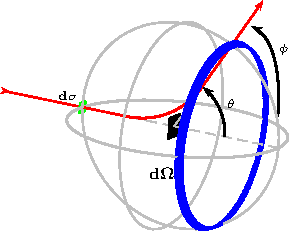
\includegraphics[width=0.8\textwidth]{./fig/compton_scattering_illustration_1.pdf}
    \caption{Showcase of solid angle $d\Omega$ and the differential size of the impact plane $d\sigma$ for $\theta=$~\unit{60}{deg}.}
    \label{fig:differential_cross_section_1}
  \end{subfigure}
  \begin{subfigure}{0.49\textwidth}
    \centering
    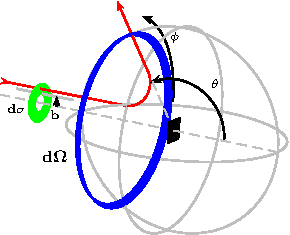
\includegraphics[width=0.8\textwidth]{./fig/compton_scattering_illustration_2.pdf}
    \caption{Showcase of solid angle $d\Omega$ and the differential size of the impact plane $d\sigma$ for $\theta=$~\unit{120}{deg}.}
    \label{fig:differential_cross_section_2}
  \end{subfigure}
  \caption{Illustration of the differential cross section for two possible values of $\theta$. The solid angle $d\Omega$ is integrated over all values of $\phi$ since the azimuthal angle $\phi$ is not changed by the scattering process.}
  \label{fig:differential_cross_section}
\end{figure}

Photon attenuation, i.e., the decrease of the intensity $d\Phi$ of an incident beam with original flux $\Phi \left[\mathrm{s}^{-1}\right]$ is described as
\begin{equation}
  \frac{d\Phi}{dz} = -n\sigma\Phi
\end{equation}
where $dz$ is the thickness of the blocking material, \unit{n_e}{\left[m^{-3}\right]} is the electron density of the material and $\sigma \left[\mathrm{m}^{2}\right]$ is the total cross section of the interaction.
By solving the differential equation, we obtain a relationship between the initial flux $\Phi$ and the remaining flux $\Phi_{out}$ behind the object with the thickness $z$:
\begin{equation}
  \Phi_{out} = \Phi e^{-n\sigma z}.
\end{equation}
This the probability of an \emph{event} (photoelectric effect, Compton scattering, etc.) $\mathrm{P}\left(E\right)$ is modeled as
\begin{equation}
  \mathrm{P}\left(E\right) = 1 - e^{-n\sigma z}.
\end{equation}

%%}

%%{ PHOTOELECTRIC EFFECT

\subsubsection{Photoelectric effect}

Photoelectric effect (Einstein, 1905) describes a total absorption of a photon by an electron.
When the electron is absorbed, the energy of the photon is completely consumed.
A portion of the energy is responsible for releasing the electron from the atomic orbital; the rest is converted to kinetic energy of the electron.

Photon energy can be expressed using its wavelength \unit{\lambda}{\left[m\right]} or frequency \unit{\nu}{\left[Hz\right]} as
\begin{equation}
  E_{\gamma} = \frac{hc}{\lambda} = h\nu,
\end{equation}
where $h \approx $ \unit{6.62 \cdot 10^{-34}}{m^2\,kg\,s^{-1}} is the Planck constant and \unit{c \approx 2.99 \cdot 10^{8}}{m\,s^{-1}} is the speed of light in a vacuum.
Let us define the ratio
\begin{equation}
  k = \frac{E_{\gamma}}{E_e}
\end{equation}
between the photon energy $E_{\gamma} = h\nu \left[\mathrm{eV}\right]$ and the electron rest mass energy \unit{E_e = m_ec^2 \approx 5.11 \cdot 10^5}{eV}.
According to \cite{fornalski2018simple}, the simplified version of the Gavrila-Pratt \cite{davisson1965interaction} cross section for the photoelectric effect is
\begin{equation}
  \label{eq:pe_cross_section}
  \sigma_{ph} = \frac{16}{3}\sqrt{2}\pi r_e^2\alpha^4\frac{Z^5}{k^{3.5}},
\end{equation}
where \unit{r_e \approx 2.81 \cdot 10^{-15}}{m} is the classical electron radius, $\alpha \approx 1/137.04$ is the fine structure constant and $Z$ is the atomic number of the element.
The accuracy of (\ref{eq:pe_cross_section}) is low even in the energy range, where it should be used ($\approx 1$ -- \unit{1000}{keV}).
To achieve better accuracy, one could build upon the work of, e.g., Gavrila-Pratt \cite{davisson1965interaction}, Scofield et al. \cite{scofield1973theoretical}, or Hubbell et al. \cite{hubbell1980pair}.
However, the cross section (\ref{eq:pe_cross_section}) will suffice for this work.

The probability of a single photoelectric effect event within a material of thickness $z$ is calculated as
\begin{equation}
  \mathrm{P}\left(E_{pe}\right) = 1 - e^{-n\sigma_{pe} z}.
\end{equation}

% Cross section $\sigma_{ph}$ for $k > 0.9$
% \begin{equation}
%   \sigma_{ph} = Z^5\left[\sum_{n=1}^4 \frac{a_n + b_nZ}{1 + c_nZ}K^{-p_n}\right],
% \end{equation}
% where {\color{red} TODO } \cite{hubbell1980pair}.
% \begin{table}
%   \centering
%   \begin{tabular}{c c c c c}
%     \hline
%     n & $a_n$ & $b_n$ & $c_n$ & $p_a$ \\
%     \hline
%     1 \rule{0pt}{2.3ex} & $1.6268 \cdot 10^{-9}$ & $-2.683 \cdot 10^{-12}$ & $4.173 \cdot 10^{-2}$ & 1 \\
%     2 & $1.5274 \cdot 10^{-9}$ & $-5.110 \cdot 10^{-13}$ & $1.027 \cdot 10^{-2}$ & 2 \\
%     3 & $1.1330 \cdot 10^{-9}$ & $-2.177 \cdot 10^{-12}$ & $2.013 \cdot 10^{-2}$ & 3.5 \\
%     4 & $-9.12 \cdot 10^{-11}$ & 0 & 0 & 4\\
%     \hline
%   \end{tabular}
%   \caption{\cite{hubbell1980pair}}
% \end{table}

%%}

%%{ COMPTON SCATTERING

\subsubsection{Compton scattering}

Compton scattering occurs when a photon transfers a portion of its energy to an electron.
During this interaction, the photon is deflected from its original path by the radial angle $\theta$ and azimuthal angle $\phi$.

The ratio $E_r$ of the energy of incoming ($E_{0}$) and scattered ($E_{s}$) particles was observed and described by Compton as
\begin{equation}
  E_r\left(\theta, E_0\right) = \frac{E_s\left(\theta, E_0\right)}{E_{0}} = \frac{1}{1 + \frac{E_0}{m_ec^2}\left(1 - \cos\theta\right)},
\end{equation}
where $\theta \in \left[-\pi, \pi\right)$ is the radial angle at which the photons are scattered, $E_0, E_s$ $\left[\mathrm{J}\right]$ are the energies of the incoming and scattered photons, \unit{m_e \approx 9.10 \cdot 10^{-31}}{kg} is the invariant mass of the electron, \unit{c \approx 2.99 \cdot 10^{8}}{m\,s^{-1}} is the speed of light in vacuum.

The Klein-Nishina formula \cite{leo2012techniques} describes the differential cross section \unit{d\sigma/d\Omega}{[m^2/sr]} of the incident and scattered beam as
\begin{equation}
  \label{eq:compton_differential_cross_section}
  \frac{d\sigma}{d\Omega}\left(\theta\right) = \frac{1}{2}\,r_{e}^2\,E_r\left(\theta\right)^2\left(E_r\left(\theta\right) + \frac{1}{E_r\left(\theta\right)} - \sin^2\theta\right),
\end{equation}
where \unit{r_e \approx 2.81 \cdot 10^{-15}}{m} is the classical electron radius.
As with the photoelectric effect, the prior probability of the scattering in a material with thickness $z$ is computed as:
\begin{equation}
  \label{eq:compton_prior}
  \mathrm{P}\left(E_{cs}\right) = 1 - e^{-n\sigma_{cs} z}.
\end{equation}
The value of likelihood probability density corresponding to the event $E_{cs}$ of a single photon with initial energy \unit{E_o}{[eV]} being scattered by the angle \unit{\theta}{[rad]} is calculated as
\begin{equation}
  \label{eq:compton_likelihood}
  \mathrm{P}\left(\theta \mid E_{cs}\right) = \frac{\int_0^{2\pi} \frac{d\sigma}{d\Omega}\,\sin \theta\,d\phi}{\sigma_{cs}},
\end{equation}
where $\sigma_{cs}$ is the total differential cross section for Compton scattering obtained from (\ref{eq:compton_differential_cross_section}).
To obtain the posterior probability density of the scattering under by the angle $\theta$, the likelihood (\ref{eq:compton_likelihood}) is multiplied by the prior probability of the Compton scattering (\ref{eq:compton_prior}):
\begin{equation}
  \mathrm{P}\left(E_{cs} \mid \theta\right) = \mathrm{P}\left(\theta \mid E_{cs}\right) \mathrm{P}\left(E_{cs}\right) = \left(1 - e^{-n\sigma_{cs} z}\right) \frac{\int_0^{2\pi} \frac{d\sigma}{d\Omega}\,\sin \theta\,d\phi}{\sigma_{cs}}.
\end{equation}

Figure~\ref{fig:compton_probs} shows the differential cross section of the Compton scattering, the likelihood of scattering by the angle $\theta$ and the posterior probability of scattering by the angle $\theta$, calculated for \unit{1}{mm} of silicon.

\begin{figure}[ht]
  \centering
  \begin{subfigure}{0.32\textwidth}
    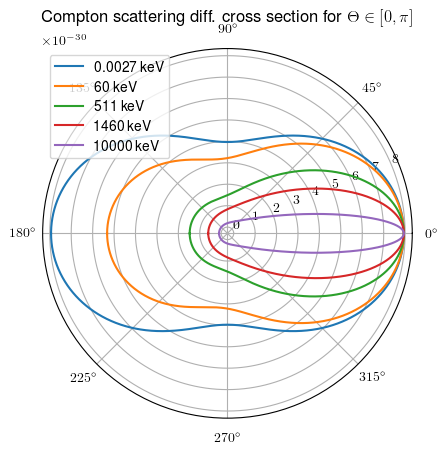
\includegraphics[width=1.0\textwidth]{./fig/klein_nishina_1.png}
    \caption{Plots of the differential cross $d\sigma/d\Omega$ section for various photon energies.}
    \label{fig:klein_1}
  \end{subfigure}
  \begin{subfigure}{0.32\textwidth}
    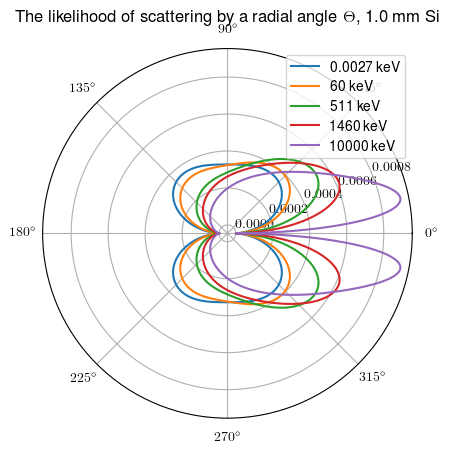
\includegraphics[width=1.0\textwidth]{./fig/klein_nishina_3.png}
    \caption{Plots of likelihood probability $\mathrm{P}\left(\theta \mid E_0\right)$, integrated over azimuthal angle $\phi$.}
    \label{fig:klein_2}
  \end{subfigure}
  \begin{subfigure}{0.32\textwidth}
    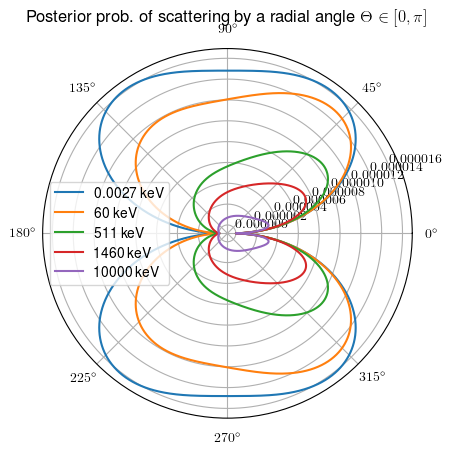
\includegraphics[width=1.0\textwidth]{./fig/klein_nishina_2.png}
    \caption{Plots of posterior probability $\mathrm{P}\left(E_0 \mid \theta\right)$, integrated over azimuthal angle $\phi$.}
    \label{fig:klein_3}
  \end{subfigure}
  \caption{Plots of the Klein-Nishina differential cross section (\ref{fig:klein_1}), the cross section normalized by the total cross section, integrate over the radial angle $\phi$ (\ref{fig:klein_2}) and the resulting probability distribution (\ref{fig:klein_3}), integrate over $\phi$.}
  \label{fig:compton_probs}
\end{figure}

% The intensity of the scattered beam \unit{N_s}{\left[s^{-1}\right]} is calculated for a small finite solid angle \unit{\Delta \theta}{\left[sr\right]} as
% \begin{equation}
%   N_s = N_o\,\frac{d\sigma}{d\Omega}\left(\theta\right)\,n_e\,t\,\Delta\theta,
% \end{equation}
% where \unit{N_0}{\left[s^{-1}\right]} is the intensity of the incoming beam, \unit{n_e}{\left[m^{-3}\right]} is the electron density of the scattering material and \unit{t}{\left[m\right]} is the effective thickness of the scattering material.

%%}

%%{ ELECTRON PAIR PRODUCTION

\subsubsection{Electron-positron pair and triplet production}

At higher energies, \unit{>1}{MeV}, the photoelectric effect and Compton scattering are dominated by the electron-positron pair and triplet productions effects \cite{hubbell1980pair}.
Since the aim of this work is to simulate the Compton camera, where only the first two effects are responsible in producing measurement, we omit the later two.
In the real sensor, the pair and triplet production would create an unwanted signal which would be filtered out by the processing software, responsible for particle track classification.

%%}

%%{ PHOTON ATTENUATION

\subsubsection{Photon attenuation}

\begin{figure}[ht]
  \centering
  \begin{subfigure}{0.49\textwidth}
    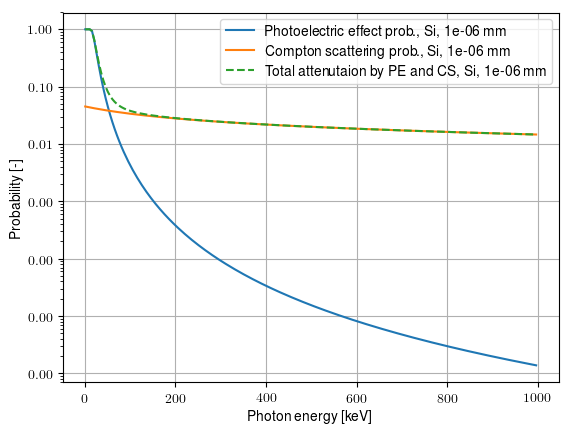
\includegraphics[width=1.0\textwidth]{./fig/scatterer_attenuation.png}
    \caption{Photon attenuation on \unit{1}{mm} of Si.}
    \label{fig:scatterer_attenuation}
  \end{subfigure}
  \begin{subfigure}{0.49\textwidth}
    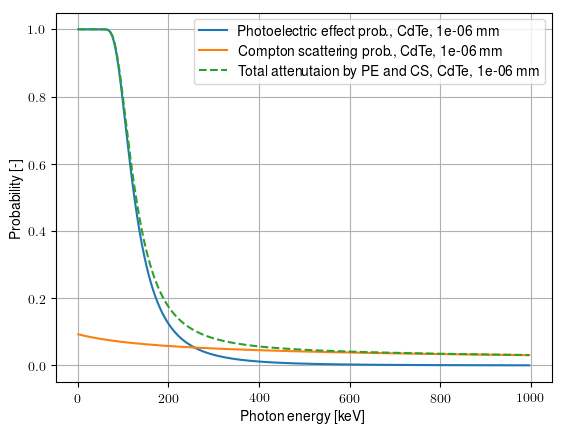
\includegraphics[width=1.0\textwidth]{./fig/absorber_attenuation.png}
    \caption{Photon attenuation on \unit{1}{mm} of CdTe.}
    \label{fig:absorber_attenuation}
  \end{subfigure}
  \label{fig:photon_attenuation}
  \caption{Photon attenuation on (\ref{fig:scatterer_attenuation}) the scatterer and (\ref{fig:absorber_attenuation}) the absorber.}
\end{figure}

%%}

%%}

%%}

\clearpage

%%%{ RADIATION SOURCE ESTIMATION

%\section{Radiation source state estimation}

%%%}

%%%{ DISTRIBUTED SENSING USING MULTIPLE UAVS

%\section{Distributed sensing using multiple UAVs}

%%%}

%%%{ AUTONOMOUS TRACKING OF A MOVING RADIATION SOURCE

%\section{Autonomous tracking of a moving radiation source}

%\subsection{Predicting target motion}

%%%}

%%%{ CONCLUSIONS

%\section{Conclusions}

%%%}

%%{ DOC BOTTOM

%%{ REFERENCES

\clearpage
\bibliography{main}{}
\cleardoublepage
\bibliographystyle{IEEEtran}
\clearpage

%%}

%%{ APENDICES

% \appendices
% \lhead{\emph{APPENDIX \leftmark}}
% \cleardoublepage

%%}

\end{document}

%%}
